
Each cable is a single Nb-Ti strand of 0.7 mm diameter with a copper stabilizer. As presented in Fig. \ref{fig:materials_cross_section}, the winding is covered with 0.007 mm thick S2-glass insulation (in red). Then, the winding is immersed in epoxy resin D10 (in blue). The superconducting cable is marked in yellow. Moreover, ground insulation is added on the external side of the coil \cite{hl_lhc_tech_design_report_v01}.

In the superconducting magnet design community, an assumption is often proposed to simulate the materials behaviour outside of the superconducting cable as a single domain characterized by the properties of G10 which is another material widely used in cryogenics. Such an assumption is made in this thesis. The characteristics of all material properties taken into consideration in the analysis are described in Appendix \ref{appendix_material_properties_description}.

\begin{figure}[H]
\centering

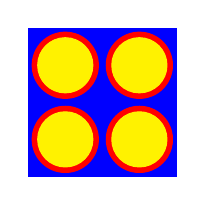
\begin{tikzpicture}[scale = 1]
\filldraw[blue] (-0.941/2,-0.941/2) rectangle (0.941/2,0.941/2);
\filldraw[red] (0,0) circle (0.7/2+0.07);
\filldraw[yellow] (0,0) circle (0.7/2);

\filldraw[blue] (-0.941/2,-0.941/2+0.941) rectangle (0.941/2,0.941/2+0.941);
\filldraw[red] (0,0+0.941) circle (0.7/2+0.07);
\filldraw[yellow] (0,0+0.941) circle (0.7/2);

\filldraw[blue] (-0.941/2+0.941,-0.941/2) rectangle (0.941/2+0.941,0.941/2);
\filldraw[red] (0+0.941,0) circle (0.7/2+0.07);
\filldraw[yellow] (0+0.941,0) circle (0.7/2);

\filldraw[blue] (-0.941/2+0.941,-0.941/2+0.941) rectangle (0.941/2+0.941,0.941/2+0.941);
\filldraw[red] (0+0.941,0+0.941) circle (0.7/2+0.07);
\filldraw[yellow] (0+0.941,0+0.941) circle (0.7/2);

\end{tikzpicture}
    \caption{Cross-section of four neighbouring windings}
    \label{fig:materials_cross_section}
\end{figure}

The stabilizer to superconductor ratio is specified in \cite{hl_lhc_tech_design_report_v01} and is calculated as follows:

\begin{equation}
    \left\{ \begin{array}{ll}
    \frac{f_\text{Cu}}{f_\text{Nb-Ti}} = \frac{A_\text{Cu}}{A_\text{Nb-Ti}} = 2.2\\ \\
    f_\text{Cu} + f_\text{Nb-Ti} = 1
    \end{array} \right.
\end{equation}

At temperatures above quench current flows through both superconductor and copper in parallel connection. What is actually quite surprising, resistivity of a superconductor above critical temperature is much higher that the one of copper. Therefore, it can be assumed that current flows through a stabilizer and only this part contributes to Joule heating. The same occurs with heat conductivity which is much lower for Nb-Ti at higher temperatures. In order to take these characteristics into account during numerical analysis, the winding area is reduced to area of copper. It leads to a formula of reduced diameter presented below.
\begin{equation}
    d_\text{strand, red} = \sqrt{\frac{A_\text{Cu}}{A_\text{strand}}}*d_\text{strand}
\end{equation}

Since the winding diameter in analysis is smaller than in reality, its equivalent heat capacity must take this correction into account which is shown in the equation below. The representative winding equivalent heat capacity is shown in Fig. \ref{fig:eq_wind_cp}.
\begin{equation}
    C_\text{p, equiv} = f_\text{Cu}*C_\text{p, Cu} + f_\text{NbTi}*C_\text{p, NbTi}
\end{equation}
 
\begin{figure}[h!]
    \centering
    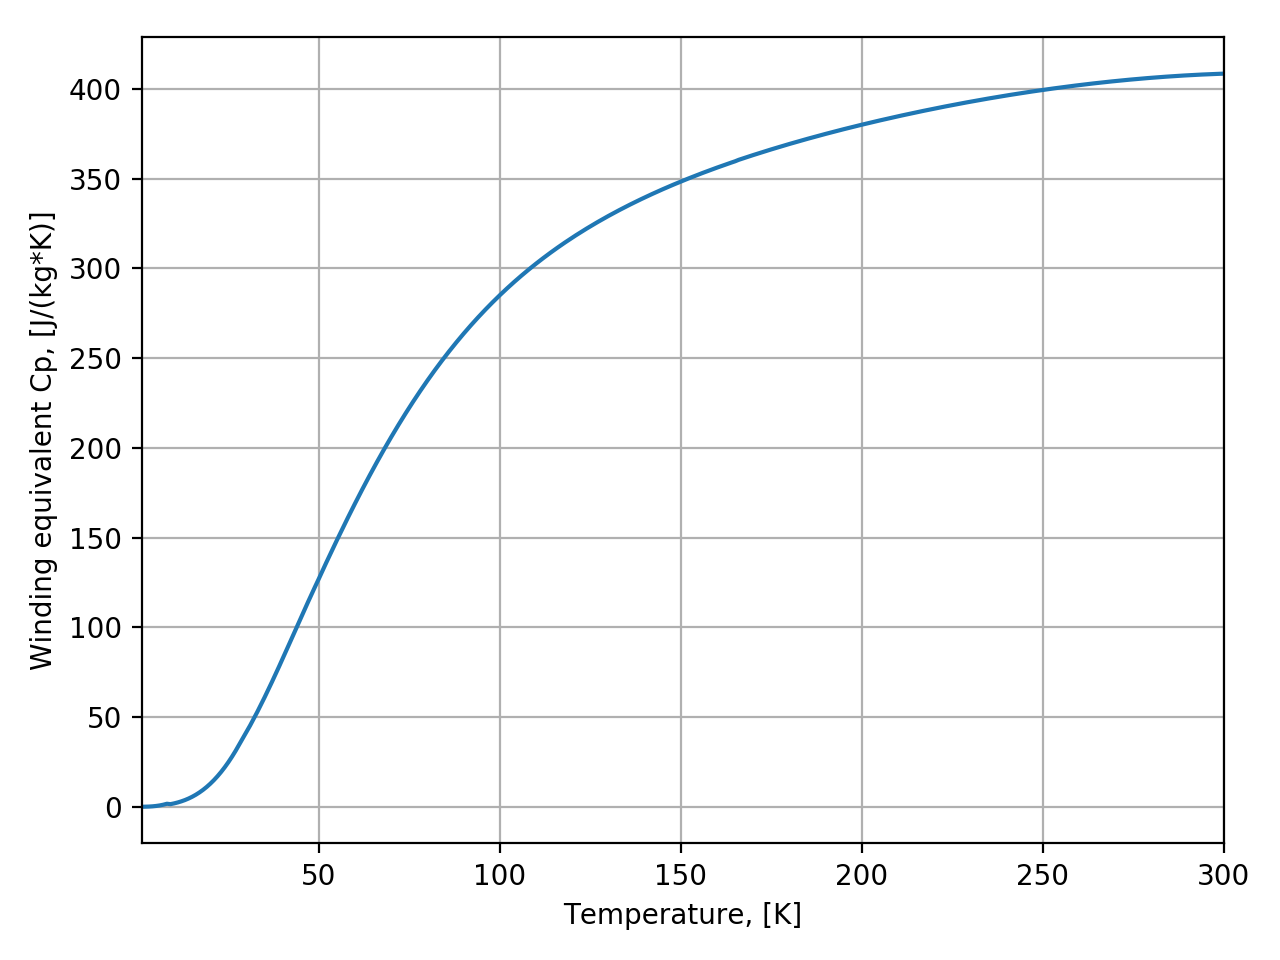
\includegraphics[width=0.35\linewidth]{figures/material_properties/Eq_Cp_plot.png}
    \caption{Equivalent winding specific heat capacity temperature dependence for \textit{B}=3 T}
    \label{fig:eq_wind_cp}
\end{figure}

The geometrical data input are collected and specified altogether in Table \ref{table:skew_quad_params_table}.

\begin{table}[h!]
    \caption{Geometrical parameters for skew quadrupole \cite{hl_lhc_tech_design_report_v01, marco_prioli_mails}} 
    \vspace{-1.em} 
    \fontsize{10}{10}
    \selectfont 
    \renewcommand{\arraystretch}{1.5}
    \begin{center}
    \begin{tabular}{ ccc }  
    \hline
    Aperture & 150 & [mm]\\
    Coil length & 841 & [m] \\
    Number of apertures & 1 & \\
    Number of circuits & 1 & \\
    Strand diameter & 0.7 & [mm] \\
    $\text{A}_\text{Cu}/\text{A}_\text{Nb-Ti}$ \cite{marco_prioli_mails} & 2.2 & \\
    \hline 
    \end{tabular}
    \end{center}  
     \label{table:skew_quad_params_table} 
 \end{table}

Insulation dimensions:

\begin{equation}
    A_\text{ins} = a^2 - \frac{\pi d_\text{strand}^2}{4}
\end{equation}

\begin{equation}
    p_\text{avg} = \frac{4 a + \pi d_\text{strand}}{2} 
\end{equation}

\begin{equation}
    L_\text{ins} = \frac{A_\text{ins}}{p_\text{avg}}
\end{equation}

\begin{equation}
    A_\text{ins,cond} = \frac{\frac{1}{4} A_\text{ins} \cdot L_{winding}}{L_\text{ins}}
\end{equation}

\begin{figure}[H]
\centering
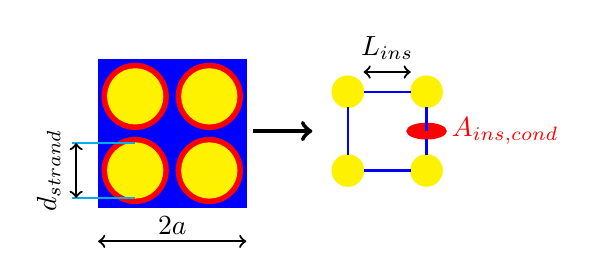
\begin{tikzpicture}[scale = 1]
\filldraw[blue] (-0.941/2,-0.941/2) rectangle (0.941/2,0.941/2);
\filldraw[red] (0,0) circle (0.7/2+0.07);
\filldraw[yellow] (0,0) circle (0.7/2);
\filldraw[blue] (-0.941/2,-0.941/2+0.941) rectangle (0.941/2,0.941/2+0.941);
\filldraw[red] (0,0+0.941) circle (0.7/2+0.07);
\filldraw[yellow] (0,0+0.941) circle (0.7/2);
\filldraw[blue] (-0.941/2+0.941,-0.941/2) rectangle (0.941/2+0.941,0.941/2);
\filldraw[red] (0+0.941,0) circle (0.7/2+0.07);
\filldraw[yellow] (0+0.941,0) circle (0.7/2);
\filldraw[blue] (-0.941/2+0.941,-0.941/2+0.941) rectangle (0.941/2+0.941,0.941/2+0.941);
\filldraw[red] (0+0.941,0+0.941) circle (0.7/2+0.07);
\filldraw[yellow] (0+0.941,0+0.941) circle (0.7/2);
\draw[thick, cyan] (-0.8,0.7/2) -- (0,0.7/2);
\draw[thick, cyan] (-0.8,-0.7/2) -- (0,-0.7/2);
\draw[black, thick, <->] (-0.75,0.7/2) -- (-0.75,-0.7/2);
\node[scale = 1, rotate=90] at (-1.1, 0) {$d_\text{strand}$};
\draw[thick,<->] (-0.941/2,-0.9) -- (0.941*1.5,-0.9);
\node[scale = 1] at (0.941*0.5, -0.7) {$2a$};
\draw[ultra thick,->, black] (1.5,0.5) -- (2.25,0.5);
\filldraw[yellow] (2.7,0) circle (0.2);
\filldraw[yellow] (3.7,0) circle (0.2);
\filldraw[yellow] (3.7,1) circle (0.2);
\filldraw[yellow] (2.7,1) circle (0.2);
\draw[thick, blue] (2.9,0) -- (3.5,0);
\draw[thick, blue] (2.9,1) -- (3.5,1);
\draw[thick, blue] (2.7,0.8) -- (2.7,0.2);
\filldraw[red] (3.7,0.5) ellipse (0.25cm and 0.1cm);
\draw[thick, blue] (3.7,0.8) -- (3.7,0.5);
\draw[thick, blue] (3.7,0.4) -- (3.7,0.2);
\draw[thick, black, <->] (2.9,1.25) -- (3.5,1.25);
\node[scale = 1] at (3.2, 1.55) {$L_\text{ins}$};
\node[scale = 1, red] at (4.7, 0.5) {$A_\text{ins,cond}$};
\end{tikzpicture}
\caption{Cross-sectional of 2D and 1D element}
\end{figure}
